\documentclass[10pt,a4paper]{report}
\usepackage[utf8]{inputenc}
\usepackage[italian]{babel}
\usepackage{amsmath}
\usepackage{amsfonts}
\usepackage{amssymb}
\usepackage{graphicx,float} % need this package
\usepackage{soul}
\usepackage{minted}
\usepackage{listings}
\newcommand{\virgolette}[1]{``#1''}

\title{Progetto Bioinformatica}
\begin{document}
\begin{figure}
 \centering
 \vspace*{-2cm} 
\includegraphics[scale=0.6]{logoUnict.jpg}
 \label{fig:logoUnict}
\end{figure}


\centerline{{\LARGE UNIVERSIT\`{A} DEGLI STUDI DI CATANIA}}
\centerline{DIPARTIMENTO DI MATEMATICA E INFORMATICA} \centerline{CORSO DI LAUREA MAGISTRALE IN INFORMATICA}
\centerline{\rule{18cm}{0.2mm}}\vspace*{2cm}
\centerline{\LARGE{BioCT}}
\centerline{\LARGE{}}
%\centerline{\LARGE{sui moderni browser: un'analisi comparativa}}\vspace*{2cm}
\vspace*{2cm}
\centerline{\rule{4cm}{0.2mm}}\medskip
\centerline{RELAZIONE PROGETTO BIOINFORMATICA}
\centerline{\rule{4cm}{0.2mm}}
\vspace*{7cm}
\begin{minipage}[t]{0.47\textwidth}
\raggedright{
\makebox[3cm][l]{Giuseppe Parasiliti W82/000152}\par
\makebox[3cm][l]{Giuseppe Sgroi W82/000131}\par}
\end{minipage}
\vspace*{2.5cm}
\begin{minipage}[t]{0.47\textwidth}
\raggedleft{
\makebox[5cm][l]

\makebox[3cm][l]
{Prof. Alfredo Ferro}\par} \vspace*{0.5cm}
\end{minipage}

\centerline{\rule{18cm}{0.2mm}} 
\centerline{ANNO ACCADEMICO 2017/2018}
\newpage
\thispagestyle{empty}

\tableofcontents
\newpage
\chapter{Introduzione}
\section{Cos'è la Bioinformatica}
La bioinformatica è una disciplina scientifica dedicata alla risoluzione di problemi biologici a livello molecolare con metodi informatici e contribuisce alla descrizione dal punto di vista quantitativo dei fenomeni biologici coinvolgendo, oltre alla biologia e all'informatica, altri campi tra cui matematica applicata, statistica, biochimica ed intelligenza artificiale.

La bioinformatica principalmente si occupa di:
\begin{itemize}
\item fornire modelli statistici validi per l'interpretazione dei dati provenienti da esperimenti di biologia molecolare e biochimica al fine di identificare tendenze e leggi numeriche,
\item generare nuovi modelli e strumenti matematici per l'analisi di sequenze di DNA, RNA e proteine al fine di creare un corpus di conoscenze relative alla frequenza di sequenze rilevanti, la loro evoluzione ed eventuale funzione,
\item organizzare le conoscenze acquisite a livello globale su genoma e proteoma in basi di dati al fine di rendere tali dati accessibili a tutti, e ottimizzare gli algoritmi di ricerca dei dati stessi per migliorarne l'accessibilità.
\end{itemize}

\section{Librerie utilizzate}
Nello sviluppo della piattaforma BioCT, abbiamo utilizzato molteplici librerie, tra le più importanti ricordiamo:
\begin{itemize}
\item Python
\begin{itemize}
\item \textbf{Flask}: è un micro-framework scritto in python che ci permette di creare un Web-Server. È basato sullo strumento Werkzeug WSGI con il motore template Jinja2. Ha licenza BSD. Più informazioni su http://flask.pocoo.org/
\item \textbf{rpy2:} L'interfaccia di alto livello di rpy2 è progettata per facilitare l'utilizzo degli script R in Python. Gli oggetti R sono esposti come istanze di classi implementate in Python, con funzioni R come metodi associati a quegli oggetti.
\end{itemize}
\end{itemize}
\begin{itemize}
\item R
\begin{itemize}
\item \textbf{LIMMA}: Pacchetto fondamentale per la ricerca di biomarcatori fornito dal linguaggio R, in particolare per la ricerca dei geni differenzialmente espressi partendo da valori di espressione determinati per mezzo di esperimenti NGS.
\item \textbf{Biobase:} è parte integrante del progetto Bioconductor ed è utilizzato in molti altri pacchetti. Biobase contiene strutture standardizzate per rappresentare dati genomici.

\item \textbf{TCGA-Assembler 2}: è un software open-source che permette automaticamente di scaricare, assemblare e processare i dati \newline TCGA (The Cancer Genome Atlas). Per scaricare i dataset ci serviremo del Modulo A che acquisice i dati pubblici TCGA dal Genomic Data Commons (GDC) dell’ U.S. National Cancer Institute. Maggiori informazioni su ( https://github.com/compgenome365/TCGA-Assembler-2 )

\end{itemize}

\end{itemize}

\section{Tumori analizzati}
I tumori presi in considerazione sono i seguenti:
\begin{itemize}
\item Thymoma (THYM)
\item Thyroid Cancer (THCA)
\item Liver Hepatocellular Carcinoma(LIHC)
\end{itemize}
\subsection{Thymoma (THYM)}
Il timoma rappresenta in assoluto il più comune dei tumori che colpiscono il timo. In genere si tratta di un tumore che cresce lentamente e solo raramente si diffonde al di fuori dell'organo di origine. 
Il sistema di classificazione Masaoka è il più ampiamente usato ed è basato sulla estenzione anatomica della malattia al momento dell’intervento. Gli stadi Masaoka si suddividono:
\begin{itemize}
\item \textbf{I}: Completamente incapsulata
\item \textbf{IIA}: Invasione Microscopica invasione attraverso la capsula all’interno del tessuto adiposo
\item \textbf{IIB}: Invasione macroscopica all’interno della capsula 
\item \textbf{III}: Invasione macroscopica negli organi adiacenti
\item \textbf{IVA}: Impianti pleurali o pericardiali 
\item \textbf{IVB}: Formazione di metastasi linfogene o ematogene in siti distanti (di tipo extra-toracico)
\end{itemize}
\newpage
\subsection{Thyroid Cancer (THCA)}
Il tumore alla tiroide(TC) è causato dall'anomalo sviluppo di alcune cellule di questa ghiandola, simile ad una farfalla, situata alla base del collo appena sotto il pomo d'Adamo. Esso si manifesta molto spesso in una forma benigna e piuttosto raramente in forme maligne (assumendo in questo caso il nome di cancro alla tiroide).
Il cancro della tiroide non è molto comune, poiché costituisce l'1-2\% di tutti i tumori, con un'incidenza di 4,1 casi ogni 100.000 abitanti per gli uomini e 12,5 nuovi casi ogni 100.000 abitanti per le donne. Secondo stime del Registro tumori italiano, nel 2012 sono stati diagnosticati 3.200 tumori tiroidei nei maschi e 10.900 nelle femmine.

La sopravvivenza è molto elevata (oltre il 90\% a 5 anni dalla diagnosi nelle forme differenziate).
Il sistema numerico classifica i tumori secondo quattro stadi:
\begin{itemize}
\item stadio 1:  il tumore è piccolo e circoscritto;
\item stadio 2 o 3:  il tumore ha invaso i linfonodi adiacenti;
\item stadio 4:  il tumore si è diffuso ad altri organi.
\end{itemize}

Secondo il sistema TNM:
\begin{itemize}
\item \textbf{T:} indica le dimensioni del tumore e comprende quattro stadi, T1 – T4;
\item \textbf{N:} indica se nei linfonodi adiacenti alla tiroide sono presenti cellule tumorali. Comprende due stadi:
\begin{itemize}
\item \textbf{N0:} assenza di cellule tumorali;
\item \textbf{N1:} presenza di cellule tumorali (N1a: nei linfonodi nel comparto centrale, N1b nei linfonodi laterali del collo)
\end{itemize}
\item \textbf{M} indica se sono presenti metastasi. Comprende due stadi:
\begin{itemize}
\item \textbf{M0:} assenza di metastasi;
\item \textbf{M1:} presenza di metastasi.
\end{itemize}
\end{itemize}

Associando gli stadi T, N e M è poi possibile definire la stadiazione complessiva della malattia.

Tutti i \textbf{tumori anaplastici} sono considerati T4, suddivisi in due stadi:
\begin{itemize}

\item \textbf{T4a:} tumore di qualsiasi dimensione confinato alla tiroide, asportabile chirurgicamente;

\item \textbf{T4b:} tumore di qualsiasi dimensione esteso oltre la capsula tiroidea, non asportabile chirurgicamente.

\end{itemize}

\newpage
\subsection{Liver Hepatocellular Carcinoma(LIHC)}
Il carcinoma epatocellulare (epatocarcinoma o HCC) è il più frequente tumore primitivo del fegato e si riscontra, nella maggior parte dei casi, in pazienti con epatopatia cronica (70-90\% dei casi di HCC), presentandosi in una forma multifocale alla diagnosi nel 75\% dei casi.
Per la stadiazione dell’HCC non esiste un sistema universalmente accettato.\newline Nel corso degli anni sono stati proposti diversi sistemi di stadiazione, quella più diffusa ha l'acronimo TNM che indicano le 3 sottoforme per cui vengono poi raggruppate "Tumore primitivo, linfonodi (node) e metastasi a distanza", è stata accertata essere migliore negli stadi iniziali del tumore. Nella figura seguente si notano i vari stadi della malattia:
\begin{center}
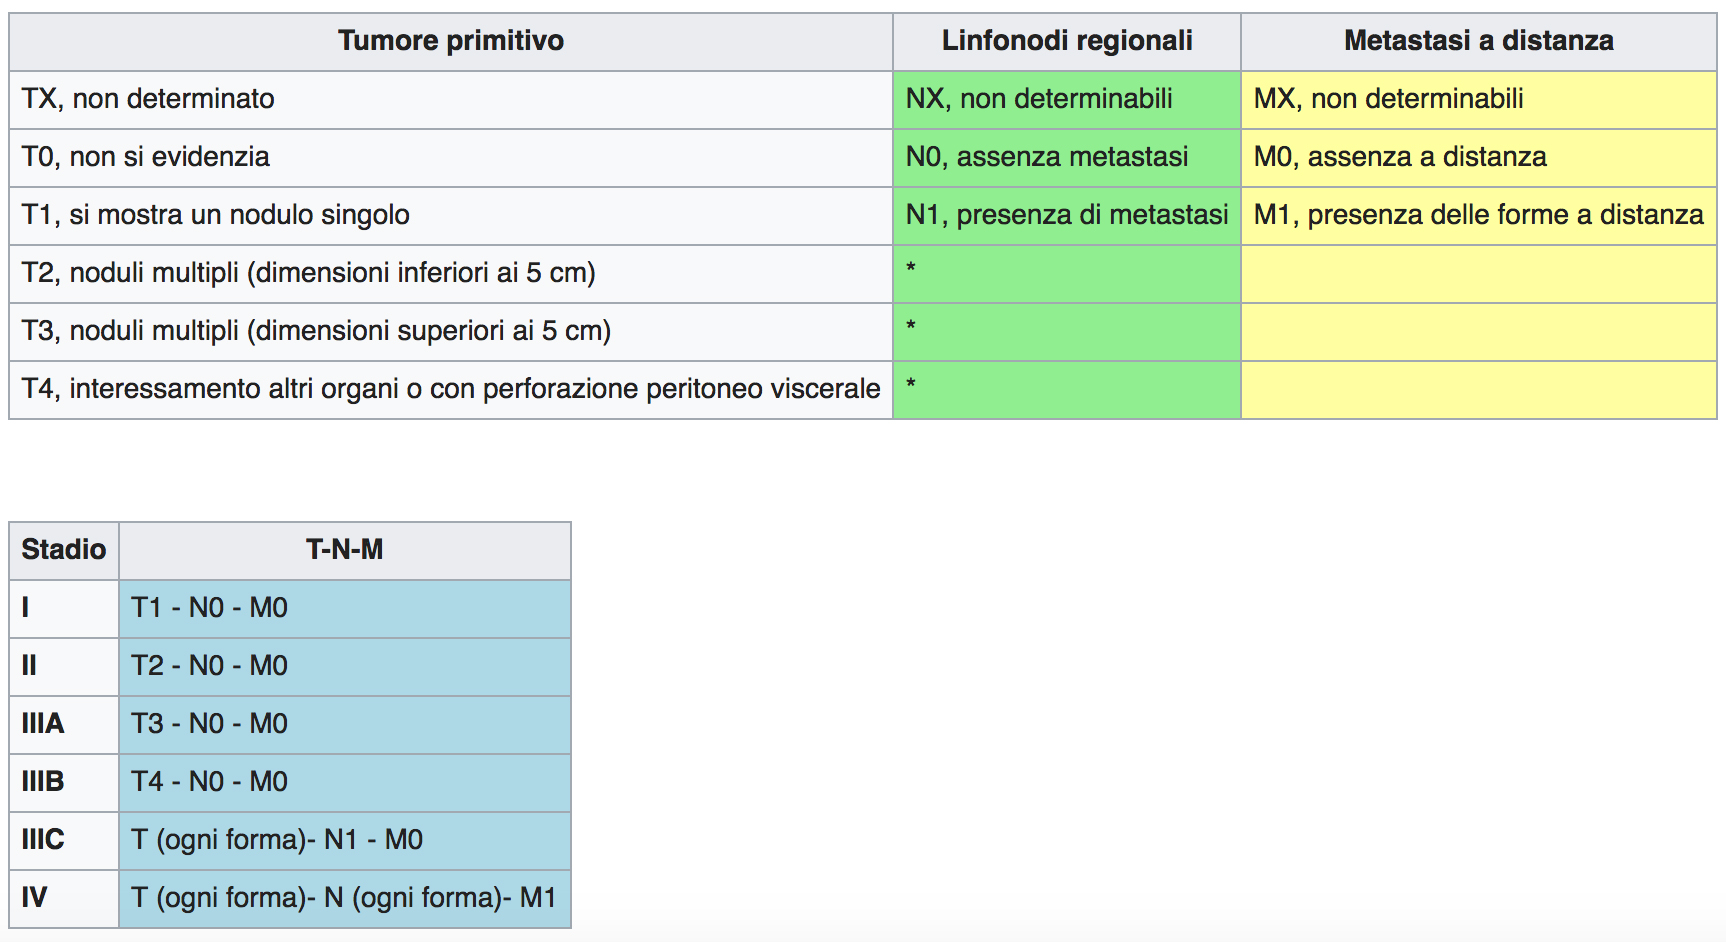
\includegraphics[scale=0.35]{stage_lihc.jpg} 
\end{center}

\chapter{BioCT}
\section{Introduzione e Funzionamento}
Obiettivo del nostro progetto è quello di realizzare un portale, da noi intitolato \textbf{“BioCT”}, che permetta all’utente finale di effettuare le analisi dei biomarcatori e la successiva interazione con Mithril nel modo più semplice e veloce possibile.
Il fulcro su cui ruota l'intero progetto è il portale \textbf{National Cancer Institute GDC Data Portal} (https://portal.gdc.cancer.gov/), dal quale estrapoliamo un set di dati specificatamente ad alcune tipologie tumorali. Per ciascun tumore estraiamo le seguenti tipologie di dati:
\begin{itemize}
\item Biospecimen \& Clinical
\item miRNA Seq.
\item RNA Seq.
\end{itemize}
Una volta salvati i dati, secondo una struttura di path ben organizzata, entriamo nel vivo dell'analisi. \newline

L’intero progetto viene eseguito tramite la libreria \textbf{Python} intitolata \textbf{\virgolette{Flask}} la quale ci permette di mettere su un Web-Server, ed è organizzato:
\begin{itemize}
\item Lato Client: molteplici pagine HTML e CSS, il cui contenuto è espresso dinamicamente in Javascript che elabora i dati in output provenienti da Python.
\item Lato Server: elaborazione dei dati attraverso Python.
\end{itemize}
\newpage
\section{Struttura}
Il progetto è strutturato in tre sezioni in ognuno delle quali viene effettuata un tipo particolare di analisi dati:
\begin{itemize}
\item \textbf{Dashboard}: schermata principale che offre la possibilità di selezionare il tumore e scaricare il dataset relativo, permettendo all’utente di scegliere di scaricare i Biospecimen \& Clinical, la sequenza RNA e/o la sequenza miRNA.
\item \textbf{Biomarcatori}: in questa sezione sarà possibile eseguire l’analisi del tumore desiderato, permettendo all’utente di scegliere i vari parametri di input.
\item \textbf{MITHrIL} : in questa schermata, si potrà avviare l’analisi con il programma MITHrIL selezionando la tipologia dei tumori e i vari contrasti del rispettivo tumore.
\end{itemize}

\subsection{Dashboard}
\begin{center}
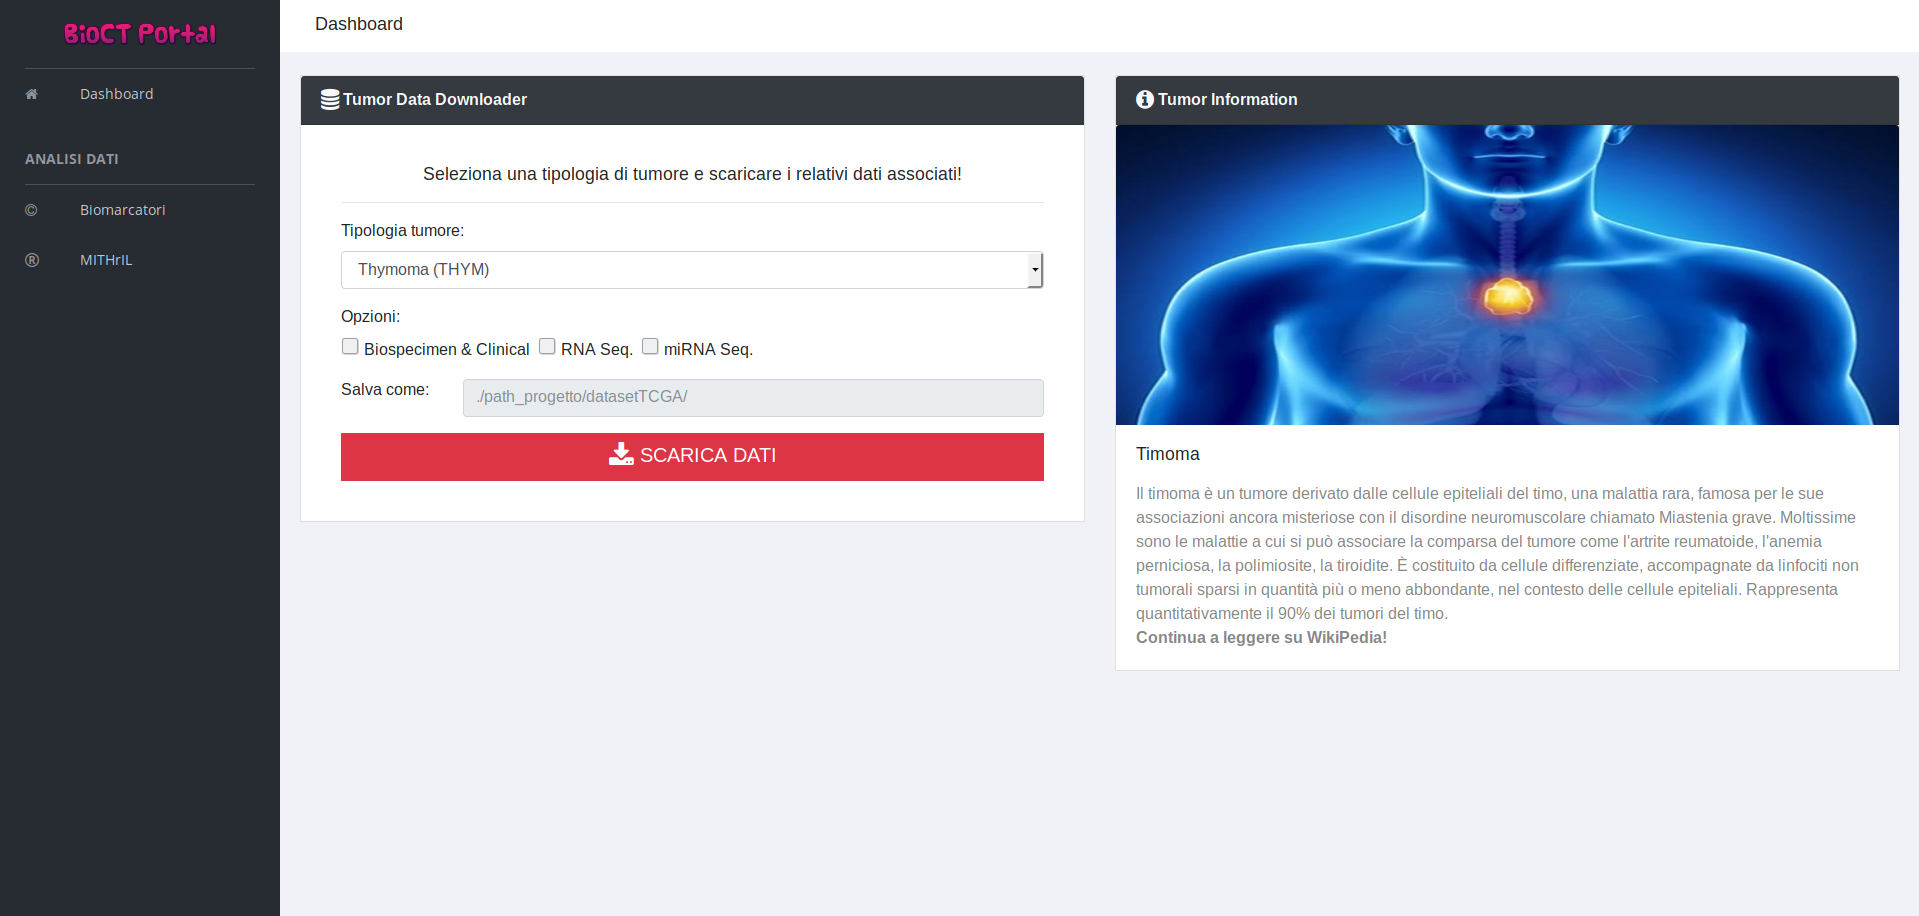
\includegraphics[scale=0.18]{Dashboard.png} 
\end{center}
In questa sezione, come già ribadito nel paragrafo precedente, è possibile selezionare il tumore di interesse e scegliere di scaricare il dataset relativo a Biospecimen \& Clinical, sequenza RNA e/o  sequenza miRNA, infine l’utente potrà scaricare i dataset selezionati cliccando su \virgolette{SCARICA DATI}. \\\\ Alla comparsa del popup, il sistema farà una chiamata POST che eseguirà lo script in python il quale creerà la cartella \virgolette{datasetTCGA} e la sottocartella relativa al tumore selezionato dall’utente, ed infine, attraverso la libreria rpy2, sopradescritta, eseguirà il codice R per scaricare i dataset attraverso la libreria sopracitata TCGA-Assembler 2. Fatto ciò si potrà procedere al download, durante il quale un popup mostrerà il processo e notificherà l’avvenuto completamento.
\subsection{Biomarcatori}
\begin{center}
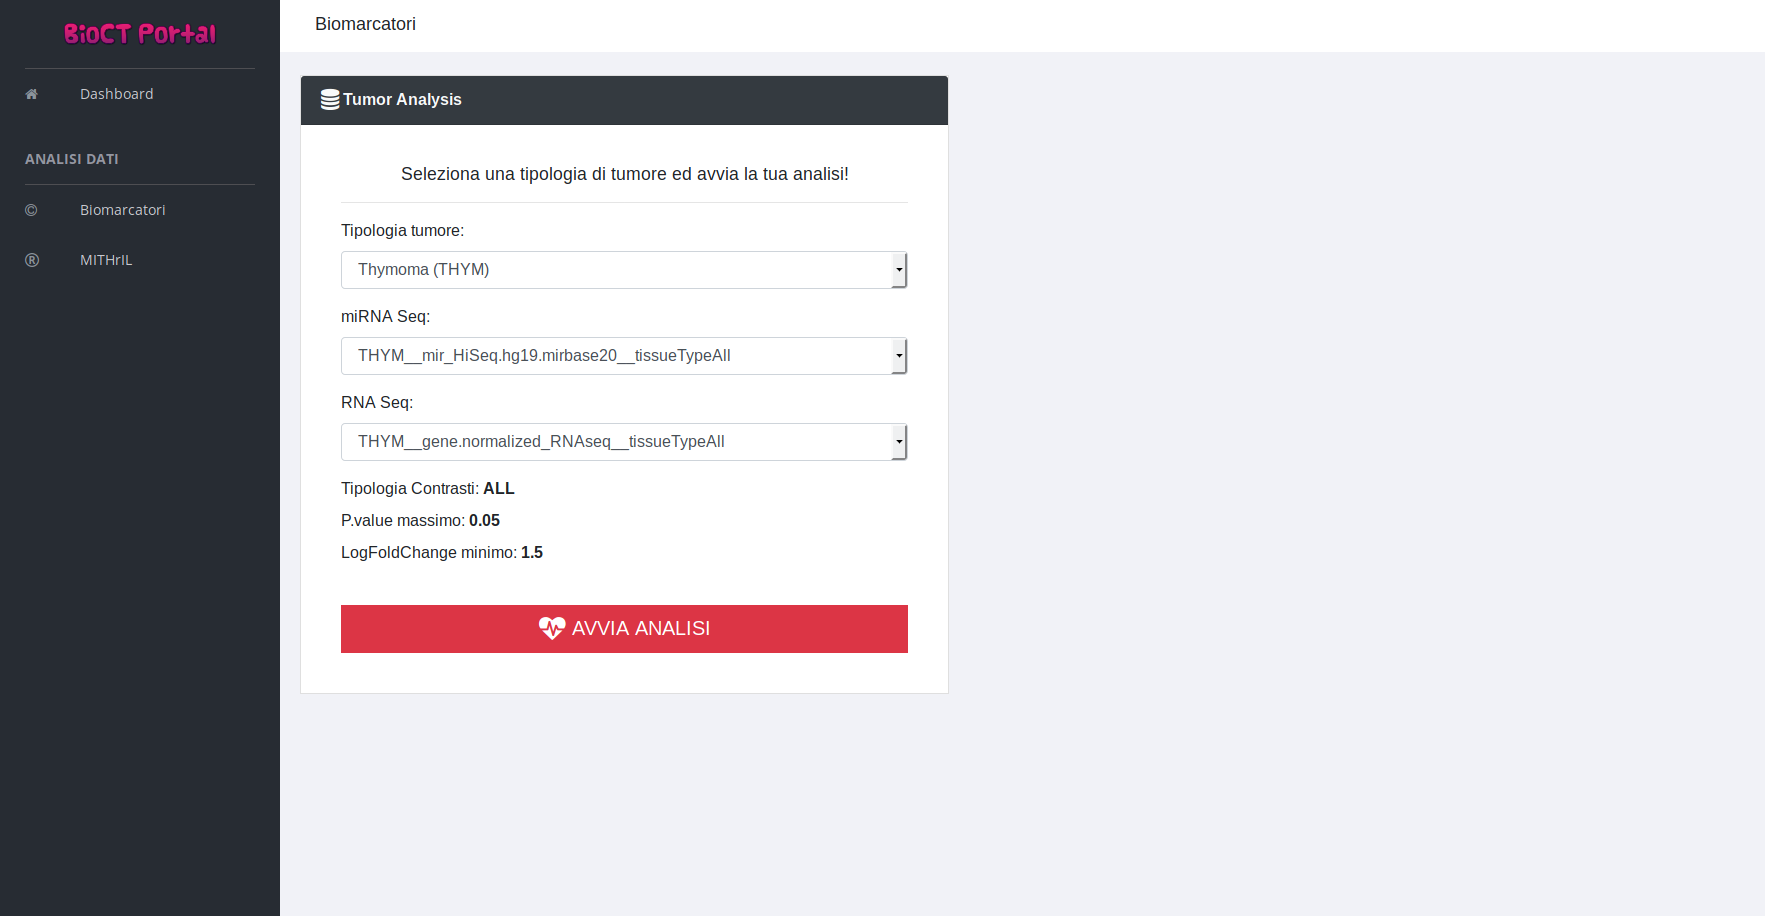
\includegraphics[scale=0.18]{Biomarcatori.png} 
\end{center}
In questa sezione l’utente può avviare l’analisi dei biomarcatori, selezionando la tipologia di tumore, scegliendo la sequenza RNA e la sequenza miRNA. L’analisi verrà avvia dopo che l’utente avrà cliccato sul bottone \virgolette{AVVIA ANALISI}, il quale attraverso una chiamata POST verrà eseguito un script in python che, dopo aver effettuato alcuni controlli sui parametri della chiamata POST, eseguirà lo script R associato al tumore selezionato dall’utente. Ultimata l’analisi iniziale dei Biomarcatori, all’utente verranno mostrati i risultati di quest’ultima così come nella figura sottostante.

\begin{figure}[H]
\centering%
\vspace{1ex}%
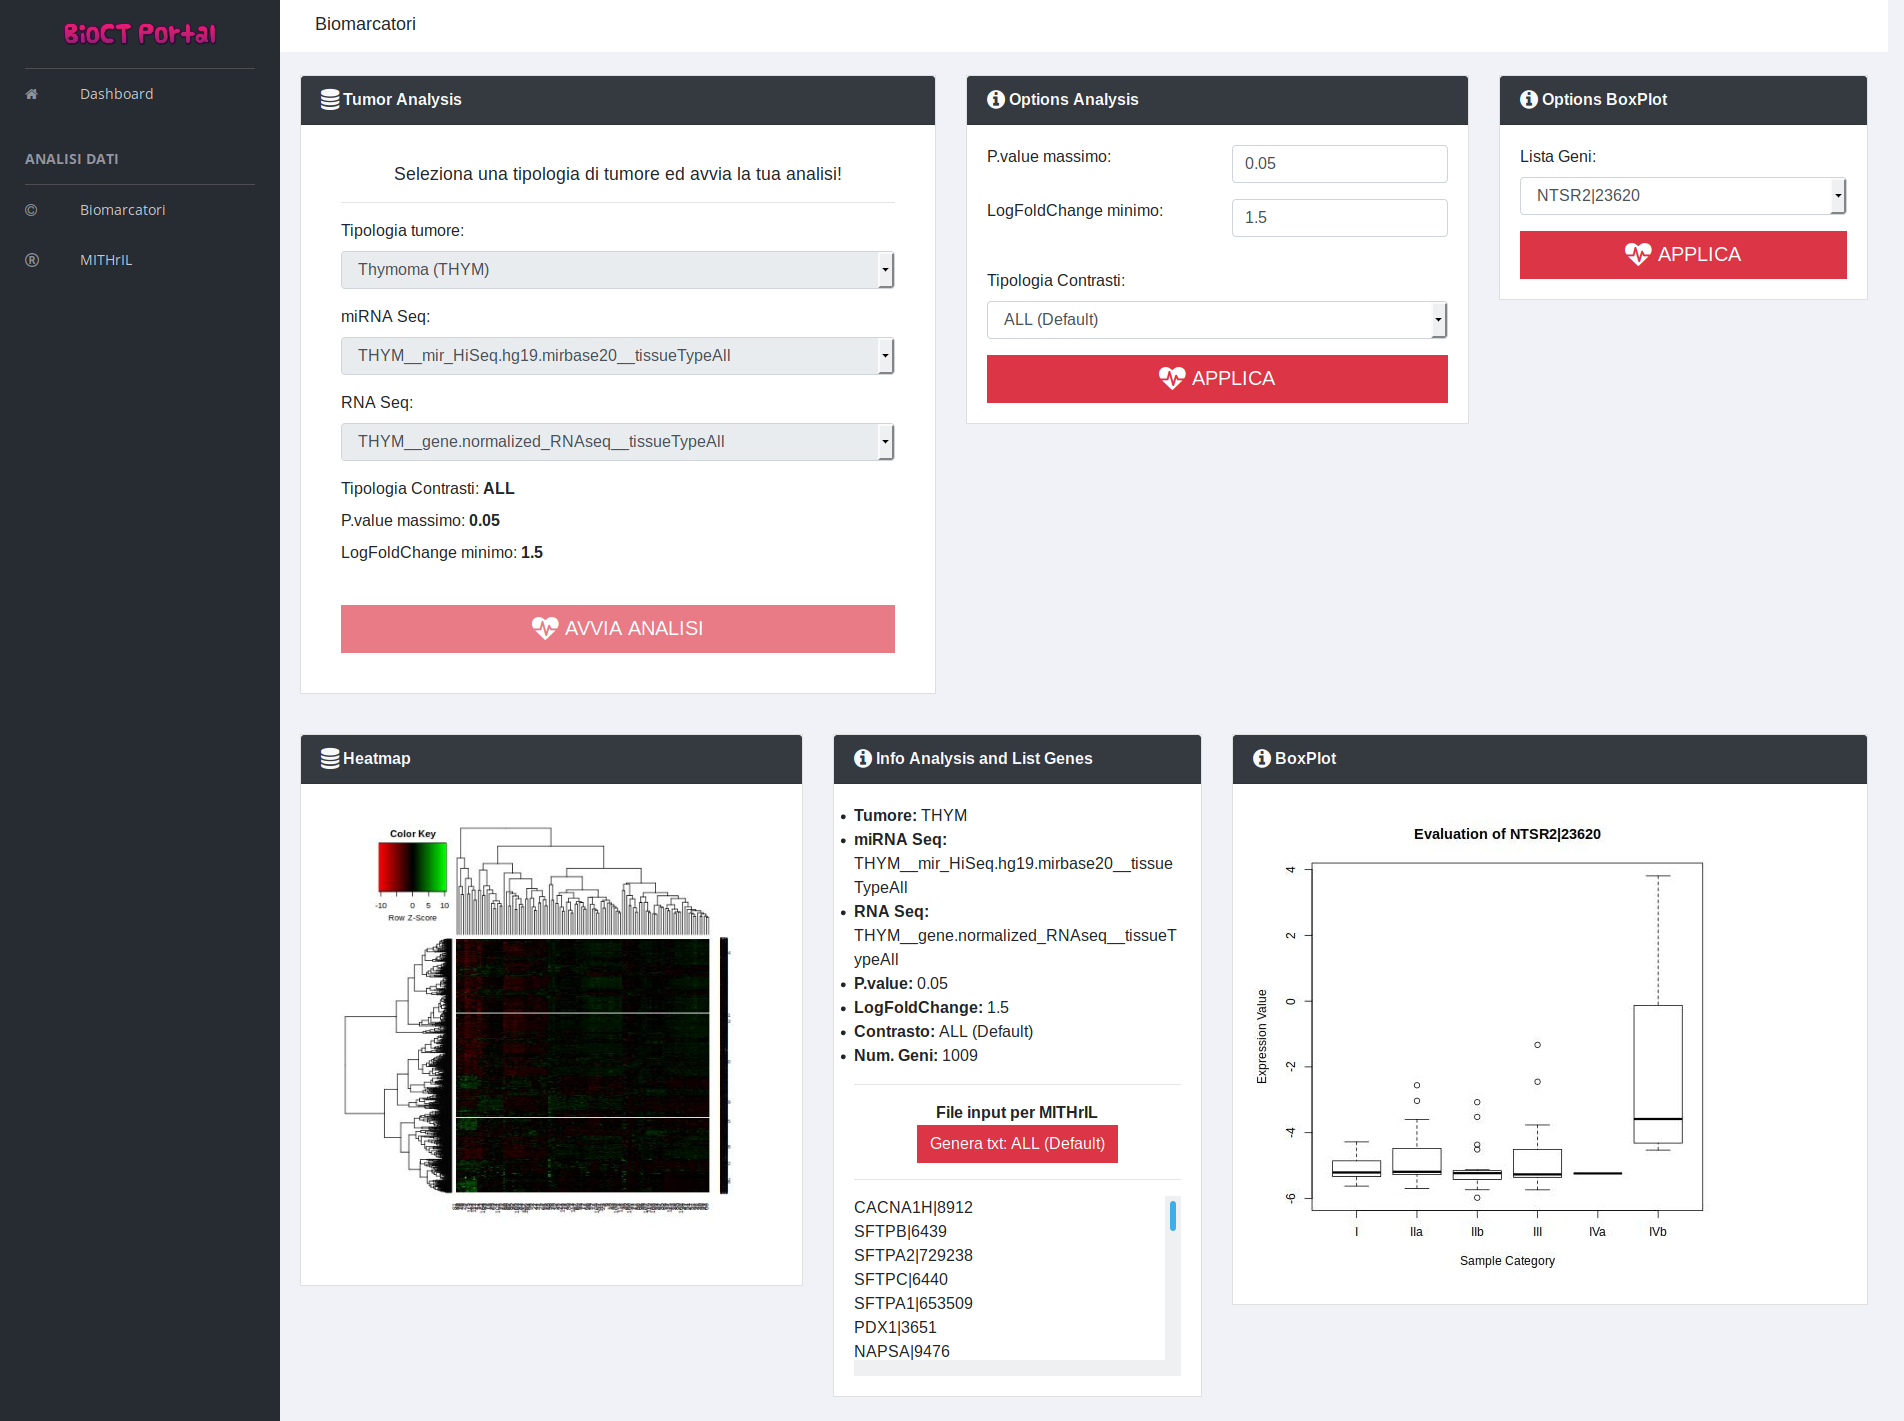
\includegraphics[scale=0.18]{Biomarcatori_1.png} 
\end{figure}
\newpage
In questa fase all’utente sono mostrati i dettagli dell’analisi da lui eseguita. Come mostrato in figura l’utente attraverso il box \textbf{\virgolette{Options Analysis}} posto al centro in alto potrà ripetere l’analisi del tumore e dei dataset relativi scelti in precedenza cambiando il valore del pvalue massimo, del LogFoldChange minimo e inoltre potrà scegliere la tipologia di contrasti\footnote{Per contrasto si intende  i vari stadi tumorali del tumore selezionato messe in relazione, secondo questa regola:  Stadio 1 vs Normale, Stadio 2 vs Stadio 1, Stadio 3 vs Stadio 2, Stadio 4 vs Stadio 3 etc.} su cui concentrarsi. \\\\ Attraverso il box \textbf{“Options BoxPlot”} in alto a destra potrà selezionare uno dei geni differenzialmente espressi estratti dall'analisi, ed automaticamente verrà generato il boxplot relativo. \newline Nel box centrale, \textbf{\virgolette{Info Analysis and List Genes}} l’utente avrà informazioni sull’analisi appena effettuata (Tumore selezionato, sequenze selezionate, pvalue, LogFoldChange, la tipologia di contrasto e il numero di geni che sono rientrati nell’analisi). All'interno dello stesso box, all'utente è data la possibilità di generare, relativamente al tumore e al tipo di contrasto selezionato, i file di input per MITHrIL.
\newpage
\subsection{MITHrIL}
MITHrIL è un metodo sviluppato per analizzare dati di espressione genica e identificare le pathway di segnalazione KEGG de-regolate dalle differenze di espressione tra i fenotipi in esame. Il metodo alla base di MITHrIL è stato descritto in un paper del 2007 di Draghici et al. \\\\ MITHrIL integra le informazioni topologiche delle pathway e dati di espressione genica per calcolare una misura di de-regolazione che definisce l’impatto di quanto osservato sulle
pathway. 

\begin{figure}[H]
\centering%
\vspace{1ex}%
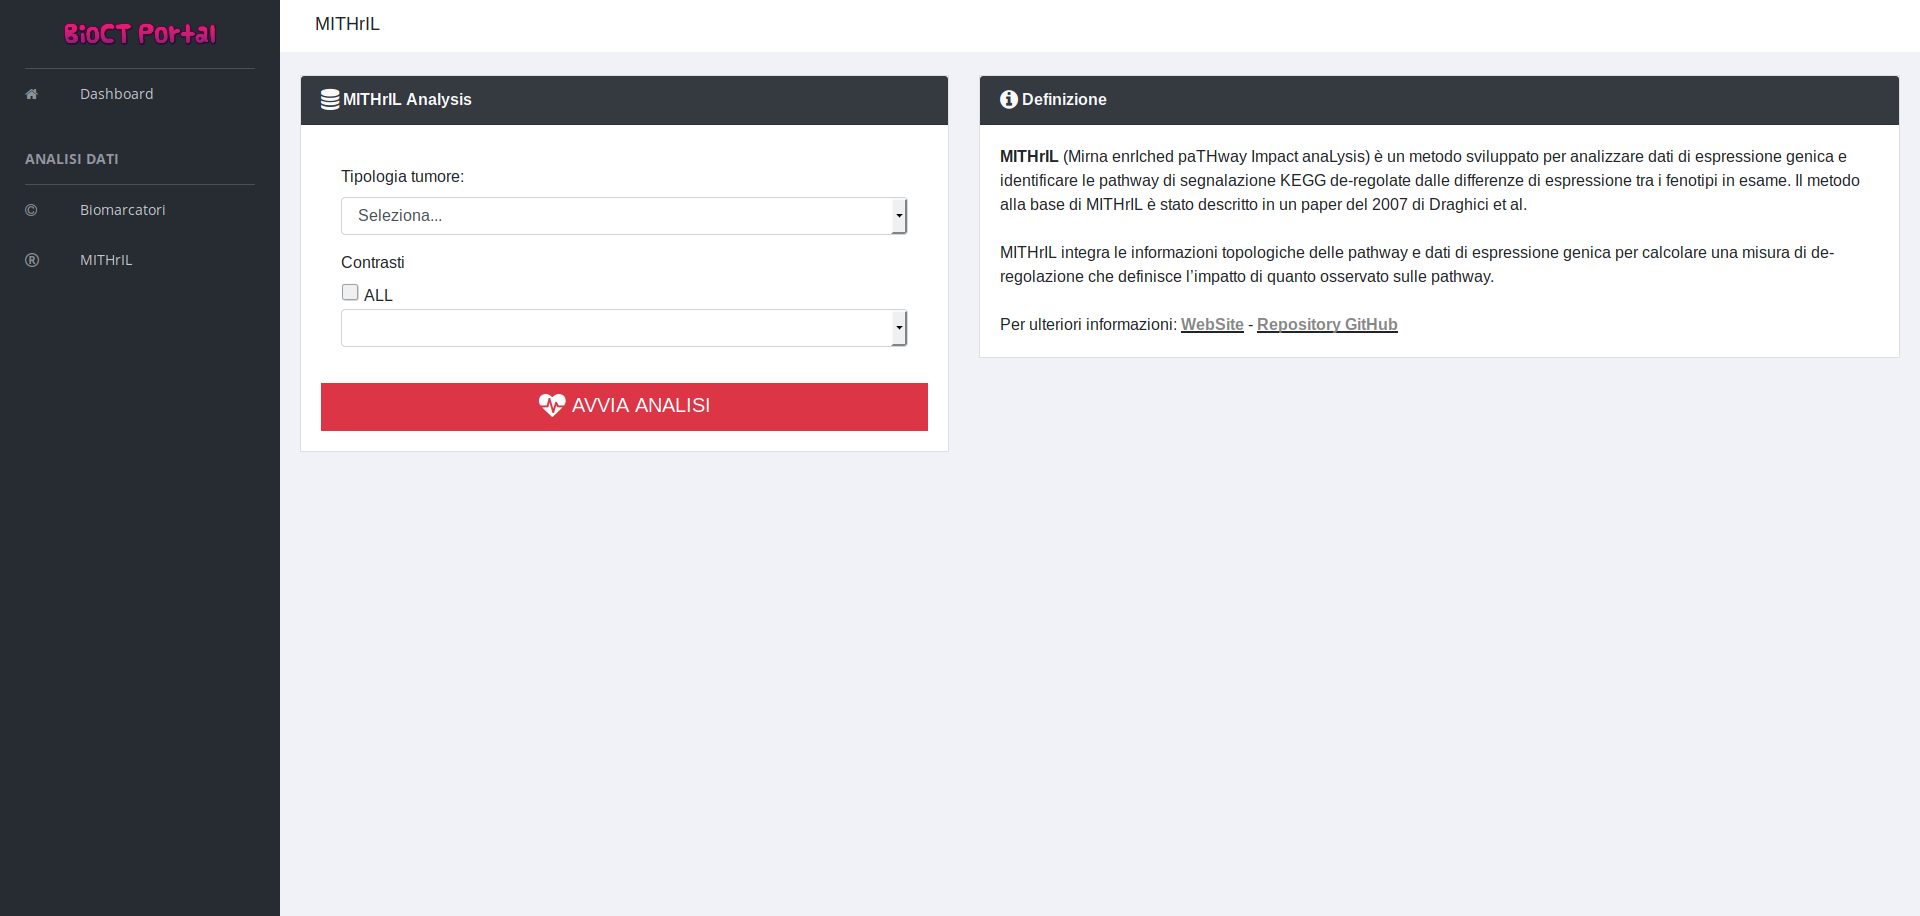
\includegraphics[scale=0.25]{mithril.png} 
\end{figure}

Generati i file di input per MITHrIL, l'utente potrà avviare l'analisi selezionado la tipologia di tumore e il contrasto che si vuole analizzare con MITHrIL. Il sistema andrà alla ricerca del file di input selezionato dall'utente e attraverso la seguente istruzione in python :

\begin{lstlisting}[frame=single, language=python]
sp.call(['java', '-jar', 'MITHrIL2.jar', 'merged-mithril',
 '-verbose', '-i', input.txt, '-o', output.txt, '-p',
  pertubations.tx])}
\end{lstlisting}
verrà avviato MITHrIL.

\newpage Se la checkbox \virgolette{ALL} viene selezionata dall'utente, esso dovrà selezionare anche il tipo di contrasto, in modo tale che automaticamente la piattaforma sceglierà la colonna relativa al contrasto selezionato dall'utente dal file contenente tutti i contrasti del relativo tumore.\\

Nel momento in cui l'utente cliccherà sul bottone \virgolette{Avvia Analisi}, verrà effettuata una chiamata POST eseguendo il codice python che permetterà di eseguire MITHrIL.\\\\Terminata l'analisi MITHrIL genererà due file: 
\begin{enumerate}
\item \textbf{out\_mithril\_TumorName\_0\_TypeContrast.txt}
\item \textbf{out\_mithril\_pertubations\_TumorName\_0\_TypeContrast.txt}
\end{enumerate}
dove:
\begin{itemize}
\item TumorName: è il nome del tumore selezionato dall'utente
\item 0: indica se l'utente ha selezionato la checkbox \virgolette{ALL}
\item TypeContrast: indica la tipologia di contrasto selezionata dall'utente.
\end{itemize}
Il primo file di output conterrà tutte le statistiche delle pathway computate da MITHrIL, il secondo file è l'output delle pertubazioni, che conterrà tutte le statistiche dei nodi computati da MITHrIL. \\\\L'utente potrà visualizzare in una tabella l'output contenente tutte le statistiche delle pathway che corrispondono al primo file output di MITHrIL (così come mostrato nella prima figura sottostante). Mentre nella seconda figura potrà visualizzare in una tabella l'output contenente tutte le statistiche delle pathway che corrispondono al file delle output delle pertubazioni.\\\\

\begin{figure}[H]
\centering%
\vspace{1ex}%
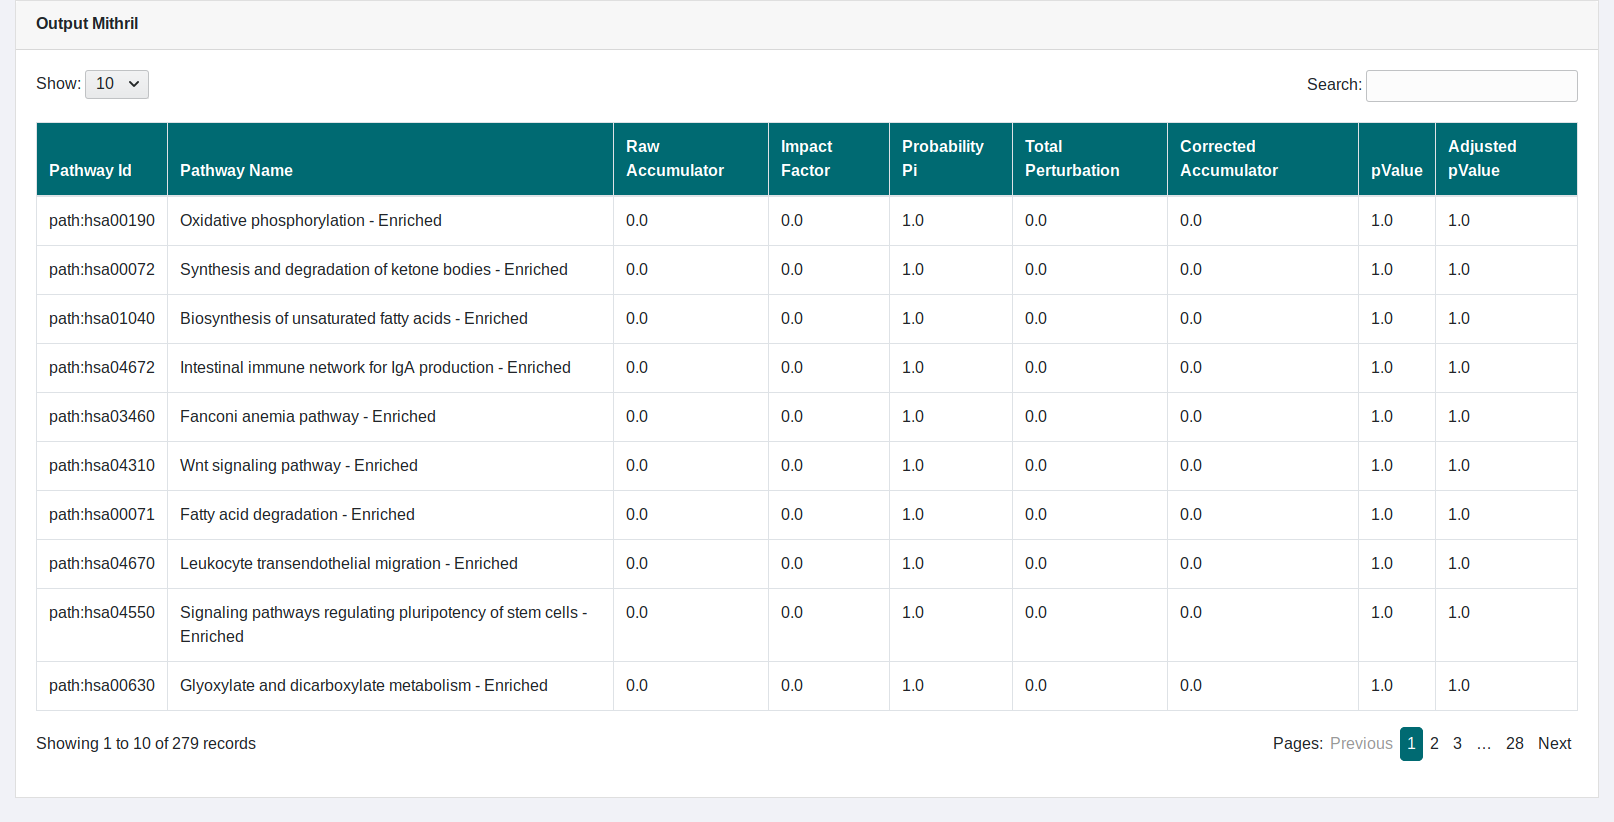
\includegraphics[scale=0.25]{outputMithril.png}  
\end{figure}

\begin{figure}[H]
\centering%
\vspace{1ex}%
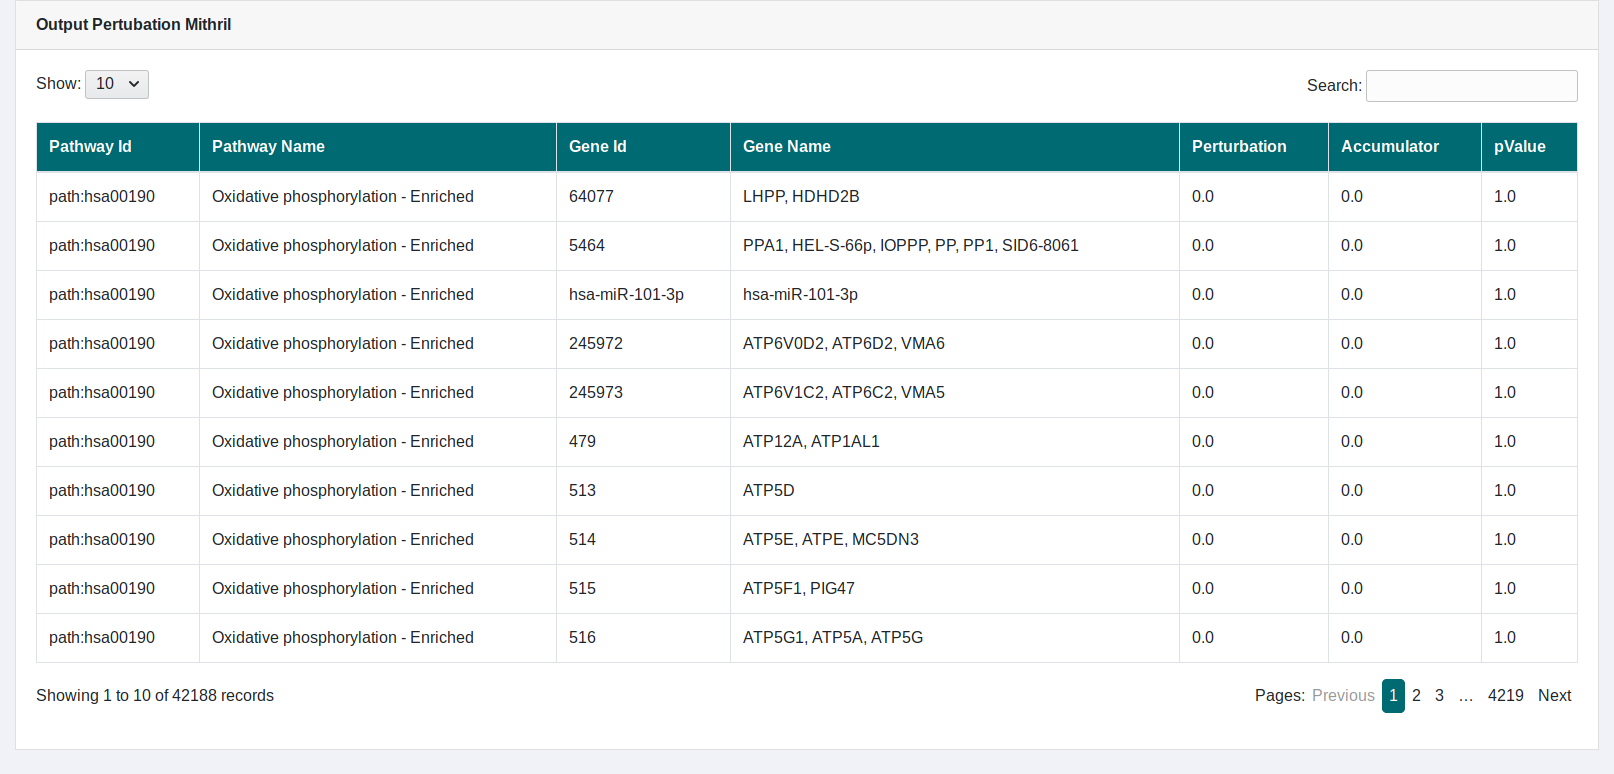
\includegraphics[scale=0.25]{outputMithrilPertubations.png}   
\end{figure}

\chapter{Guida all'utilizzo}

\begin{enumerate}
\item Importare il progetto (sviluppato su PyCharm)
\item Installare le opportune librerie richieste da R e Python
\item Aprire il file “main.py” ed avviarlo con PyCharm o IDE alternativo, oppure da un terminale eseguire il seguente comando:
\begin{minted}{bash} 
python3.6 main.py 
\end{minted}
\begin{enumerate}
\item Il web server sarà completamente avviato quando apparirà a video la seguente schermata:

\begin{figure}[H]
\centering%
\vspace{1ex}%
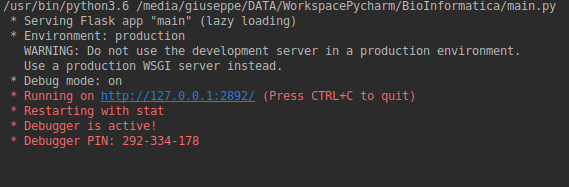
\includegraphics[scale=0.75]{pycharm.png} 
\end{figure}

\item Fare click sull’url localhost, in blu nell’immagine sovrastante, oppure inserirlo manualmente nel proprio browser. Si aprirà automaticamente il browser con la Dashboard iniziale della piattaforma BioCT.
\end{enumerate}

\end{enumerate}

\end{document}